% Fuente única de clase: Recursos/2025-10-02.pdf, páginas 1--13.
% P13 está en blanco; se revisó completa junto con las otras doce páginas.
En la clase 13 calculamos ejemplos de cocientes de polinomios y caracterizamos ideales primos y maximales. Después interpretamos los módulos como acciones de anillos sobre grupos abelianos e introducimos las álgebras sobre un anillo conmutativo.

%%%%%%%%%%%%%%%%%%%%%%%%%%%%%%%%%%%%%%%%%%%%%%%%%%%%%%%%%%%%%%%%%%%%%%%%%%%%%%%
\section{Cocientes de polinomios e ideales primos}
%%%%%%%%%%%%%%%%%%%%%%%%%%%%%%%%%%%%%%%%%%%%%%%%%%%%%%%%%%%%%%%%%%%%%%%%%%%%%%%
%%%%%%%%%%%%%%%%%%%%%%%%%%%%%%%%%%%%%%%%%%%%%%%%%%%%%%%%%%%%%%%%%%%%%%%%%%%%%%%
\subsection{Evaluación y la construcción de los complejos}
%%%%%%%%%%%%%%%%%%%%%%%%%%%%%%%%%%%%%%%%%%%%%%%%%%%%%%%%%%%%%%%%%%%%%%%%%%%%%%%
% P01--P02: repetición de IV.4.6, ejemplo IV.4.7 y cálculo con x^2+1.
En esta sección los anillos son conmutativos. La \cref{prop:C12-restos}, recordada al inicio de la pizarra, identifica el grupo aditivo de un cociente por un mónico con los coeficientes de sus restos. La multiplicación depende del polinomio usado para reducirlos.

\begin{ejem}[El resto al dividir por $x-a$]\label{ejem:C13-evaluacion}
Para $a\in R$, la división por $x-a$ tiene resto constante:
\[
g(x)=(x-a)q(x)+r.
\]
Evaluando en $a$, $g(a)=(a-a)q(a)+r=r$. Por tanto, $g(a)=0$ si y sólo si $g\in(x-a)$. La evaluación $\ev_a:R[x]\to R$ preserva suma, producto y unidad y es sobreyectiva, porque todo elemento es valor de un polinomio constante. Su núcleo es $(x-a)$, de modo que
\[
R[x]/(x-a)\cong R
\]
como \emph{anillos}, por el \cref{teo:C12-primer-iso}.
\end{ejem}

\begin{ejem}[El cociente por $x^2+1$]
Todo elemento de $R[x]/(x^2+1)$ tiene un único representante $a_0+a_1x$. Para calcular el producto escribimos
\[
\begin{aligned}
(a_0+a_1x)(b_0+b_1x)
&=a_0b_0+(a_0b_1+a_1b_0)x+a_1b_1x^2\\
&=a_1b_1(x^2+1)+(a_0b_0-a_1b_1)+(a_0b_1+a_1b_0)x.
\end{aligned}
\]
Así, al transportar el producto al grupo $R\oplus R$, se obtiene
\[
(a_0,a_1)\cdot(b_0,b_1)
=(a_0b_0-a_1b_1,\ a_0b_1+a_1b_0).
\]
Para $R=\mathbb R$, la correspondencia $(a_0,a_1)\mapsto a_0+a_1i$ respeta exactamente la multiplicación usual de complejos y es biyectiva. Por ello
\[
\mathbb R[x]/(x^2+1)\cong\mathbb C
\]
como anillos. En particular, la relación $x^2=-1$ en el cociente produce esa estructura a partir de polinomios reales.
\end{ejem}

%%%%%%%%%%%%%%%%%%%%%%%%%%%%%%%%%%%%%%%%%%%%%%%%%%%%%%%%%%%%%%%%%%%%%%%%%%%%%%%
\subsection{Primalidad, maximalidad y correspondencia}
%%%%%%%%%%%%%%%%%%%%%%%%%%%%%%%%%%%%%%%%%%%%%%%%%%%%%%%%%%%%%%%%%%%%%%%%%%%%%%%
% P03--P04.
\begin{defi}
Un ideal \emph{propio} $I\subsetneq R$ es \emph{primo} si $R/I$ es un dominio entero y es \emph{maximal} si $R/I$ es un campo. Todo ideal maximal es primo, porque todo campo es dominio.
\end{defi}

\begin{ejem}
El ideal $(x-a)$ de $R[x]$ es primo si y sólo si $R$ es dominio, y maximal si y sólo si $R$ es campo, por el \cref{ejem:C13-evaluacion}. Además, $(x^2+1)$ es maximal en $\mathbb R[x]$, porque el cociente es $\mathbb C$.

En $\mathbb Z[x]$, $(2,x)$ es maximal. En efecto, si $\bar2=2+(x)$, el ejemplo de cocientes sucesivos de la clase 12 da
\[
\mathbb Z[x]/(2,x)
\cong (\mathbb Z[x]/(x))/(\bar2)
\cong\mathbb Z/(2),
\]
que es campo. La barra recuerda que en el cociente intermedio se genera un ideal con la \emph{clase} de $2$, y no con un entero considerado fuera de ese anillo.
\end{ejem}

\begin{lema}\label{lema:C13-campo}
Un anillo conmutativo $T\ne0$ es campo si y sólo si no tiene ideales distintos de $(0)$ y $T$.
\end{lema}
\begin{proof}
Si $T$ es campo y $J\ne(0)$, elegimos $a\ne0$ en $J$. Como $a^{-1}a=1\in J$, resulta $J=T$. Recíprocamente, para cualquier $a\ne0$, el ideal $(a)$ no es cero y debe ser todo $T$. Existe $b$ con $ba=1$, y la conmutatividad hace de $b$ un inverso bilateral. Luego $T$ es campo.
\end{proof}

\begin{prop}\label{prop:C13-criterios}
Sea $I$ un ideal propio de un anillo conmutativo $R$.
\begin{enumerate}[label=\textup{(\roman*)}]
\item $I$ es primo si y sólo si, para todo $a,b\in R$, $ab\in I$ implica $a\in I$ o $b\in I$.
\item $I$ es maximal si y sólo si todo ideal $J$ con $I\subseteq J\subseteq R$ es $I$ o $R$.
\end{enumerate}
\end{prop}
\begin{proof}
El cociente $R/I$ es conmutativo y no nulo, pues $I$ es propio. La igualdad $(a+I)(b+I)=I$ equivale a $ab\in I$, y una de esas clases es cero si y sólo si su representante pertenece a $I$. Esto demuestra (i).

Por el \cref{lema:C12-correspondencia}, los ideales de $R/I$ son exactamente los $J/I$ con $J\supseteq I$. El ideal cero corresponde a $J=I$ y el ideal total a $J=R$. El \cref{lema:C13-campo} demuestra (ii).
\end{proof}
\begin{nota}[Hipótesis en el criterio de campo]
La frase manuscrita al final de la página 3 debe entenderse para un anillo \emph{no nulo}, con dos ideales distintos $(0)$ y $(1)$. El anillo cero no es campo. En la vuelta de la demostración se usa $(a)=(1)$ sólo para $a\ne0$, aunque allí se escribe «para todo $a\in R$»; para $a=0$ se tiene $(a)=(0)$.
\end{nota}

\begin{prop}\label{prop:C13-primo-maximal}
Sea $I$ un ideal propio de un anillo conmutativo $R$.
\begin{enumerate}[label=\textup{(\roman*)}]
\item Si $R/I$ es finito, $I$ es primo si y sólo si es maximal.
\item Si $R$ es DIP e $I\ne(0)$, $I$ es primo si y sólo si es maximal.
\end{enumerate}
\end{prop}
\begin{proof}
La primera afirmación es la \cref{prop:C11-finito} aplicada al cociente. Para (ii), sólo falta probar que un primo no nulo es maximal. Escribimos $I=(a)$ con $a\ne0$. Si $I\subseteq J$, escribimos $J=(b)$ y, como $a\in(b)$, tenemos $a=bc$. La primalidad de $(a)$ da $b\in(a)$ o $c\in(a)$.

Si $b\in(a)$, entonces $J\subseteq I$, luego $J=I$. Si $c=da$, la igualdad $a=bc=bda$ da $(1-bd)a=0$. Como $R$ es dominio y $a\ne0$, $bd=1$. Así, $b$ es unidad y $J=R$. Por la \cref{prop:C13-criterios}, $I$ es maximal.
\end{proof}

%%%%%%%%%%%%%%%%%%%%%%%%%%%%%%%%%%%%%%%%%%%%%%%%%%%%%%%%%%%%%%%%%%%%%%%%%%%%%%%
\subsection{Espectros de enteros y polinomios}
%%%%%%%%%%%%%%%%%%%%%%%%%%%%%%%%%%%%%%%%%%%%%%%%%%%%%%%%%%%%%%%%%%%%%%%%%%%%%%%
% P04--P06.
\begin{defi}
El \emph{espectro} de un anillo conmutativo es el conjunto de sus ideales primos:
\[
\Spec R=\set{I\subsetneq R\given I\text{ es ideal primo}}.
\]
\end{defi}
No se introduce aquí una topología; los dibujos representan las inclusiones entre ideales.

En $\mathbb Z$, para $n>0$, el ideal $(n)$ es primo si y sólo si es maximal, y esto ocurre si y sólo si $n$ es primo como entero. El ideal $(1)$ no es propio. Además, $(0)$ es primo porque $\mathbb Z$ es dominio, y no es maximal porque $\mathbb Z$ no es campo. Como todos los ideales son principales,
\[
\Spec\mathbb Z=\{(0)\}\cup\set{(p)\given p\text{ primo positivo}}.
\]
Cada $(p)$ contiene a $(0)$, y no hay inclusiones entre dos ideales maximales distintos.

\begin{ejer}[Los polinomios sobre un campo forman un DIP]\label{ejer:C13-Kx}
Probar que, si $K$ es un campo, $K[x]$ es un dominio de ideales principales. La página 5 desarrolla esta comprobación y el fragmento de la página 6 remite a ella como ejercicio IV.4.4.
\end{ejer}
\begin{sol}
El producto de dos polinomios no nulos tiene coeficiente principal igual al producto de sus coeficientes principales, que es no nulo en el campo. Así, $K[x]$ es dominio.

El ideal cero es principal. Si $I\ne(0)$, los grados de sus polinomios no nulos forman un conjunto no vacío de enteros no negativos. Elegimos $f\in I$ de grado mínimo $d$. Si $d=0$, $f$ es una constante no nula y es unidad, de modo que $I=K[x]=(1)$. Si $d\geq1$, multiplicamos $f$ por el inverso de su coeficiente principal y suponemos que es mónico.

Para $g\in I$, la \cref{prop:C12-division} da $g=fq+r$, con $\deg r<d$. Como $f,g\in I$, también $r=g-fq\in I$. Si $r\ne0$, contradice la minimalidad de $d$. Luego $r=0$, así que $g\in(f)$ y $I\subseteq(f)$. La inclusión opuesta se sigue de $f\in I$. Por tanto, $I=(f)$.
\end{sol}
\begin{nota}[Grado mínimo y signo del resto]
En la página 5, el caso posterior a $d=0$ está escrito como $d>1$; debe incluir $d=1$. En la misma prueba, de $g=fq+r$ se obtiene $r=g-fq$, mientras que la pizarra escribe $r=fq-g$. El signo no altera la pertenencia al ideal, pero sí la igualdad que define el resto. También se consideran sólo polinomios no nulos al tomar el grado mínimo.
\end{nota}

En consecuencia, los primos no nulos de $K[x]$ son maximales por la \cref{prop:C13-primo-maximal}. El ideal $(0)$ es primo y no maximal: $K[x]$ es dominio y $x$ no tiene inverso polinómico, porque los grados de productos no nulos se suman.

\begin{defi}
Un campo es \emph{algebraicamente cerrado} si todo polinomio no constante con coeficientes en él tiene una raíz en el campo. Un polinomio no nulo y no unidad es \emph{irreducible} si, en toda factorización suya, al menos uno de los factores es unidad.
\end{defi}
El fragmento afirma, sin demostrarlo aquí, que $\mathbb C$ es algebraicamente cerrado. Usamos ese hecho en la comprobación siguiente, tal como pide el texto, sin incorporar una prueba del teorema fundamental del álgebra.

\begin{ejer}[{Ideales maximales de $\mathbb C[x]$}]\label{ejer:C13-complejos}
Suponiendo que $\mathbb C$ es algebraicamente cerrado, demostrar que los ideales maximales de $\mathbb C[x]$ son exactamente $(x-z)$, $z\in\mathbb C$. Es el ejercicio IV.4.21 citado en la página 6.
\end{ejer}
\begin{sol}
Cada $(x-z)$ es maximal porque su cociente es $\mathbb C$. Recíprocamente, un maximal $M$ no puede ser $(0)$, como acabamos de ver. Por el \cref{ejer:C13-Kx}, $M=(f)$ con $f$ no nulo y no constante: una constante no nula generaría todo el anillo.

El polinomio $f$ debe ser irreducible. Si $f=gh$ con ambos factores no unidades, sus grados son positivos y menores que $\deg f$, de modo que
\[
(f)\subsetneq(g)\subsetneq\mathbb C[x],
\]
contradiciendo la maximalidad. Como $\mathbb C$ es algebraicamente cerrado, existe $z$ con $f(z)=0$. El \cref{ejem:C13-evaluacion} da $f=(x-z)q$. La irreducibilidad obliga a que $q$ sea unidad, es decir, una constante no nula. Por tanto, $(f)=(x-z)$.

Además, distintos valores dan distintos ideales: si $(x-z)=(x-w)$, entonces $x-w$ se anula en $z$, de donde $z=w$.
\end{sol}
\begin{nota}[Generador mónico e irreducibilidad]
La última línea manuscrita de la página 6 identifica los polinomios irreducibles de $\mathbb C[x]$ con los de la forma $x-z$. La afirmación literal requiere normalizar el coeficiente principal: en general son $c(x-z)$ con $c\ne0$. Por ejemplo, $2x$ también es irreducible. Todos ellos generan el mismo ideal que su representante mónico.
\end{nota}

Así, $\Spec\mathbb C[x]=\{(0)\}\cup\set{(x-z)\given z\in\mathbb C}$. La figura conserva los dos esquemas de las páginas 4 y 6: un nivel de ideales maximales, todos sobre $(0)$. En el segundo dibujo el plano sólo organiza los parámetros complejos; las líneas indican inclusiones de ideales.
% Esquemas de Recursos/2025-10-02.pdf, páginas 4 y 6.

% Una misma caja horizontal mantiene alineados los centros de ambos esquemas.
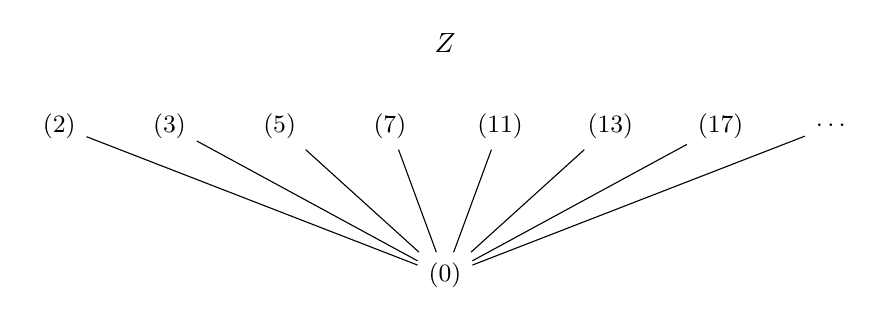
\begin{tikzpicture}[font=\small,inner sep=3pt,outer sep=1pt]
\useasboundingbox (-5.3,-.25) rectangle (5.3,3.15);
\node[font=\normalsize] at (0,2.95) {$\Spec\mathbb Z$};
\node (cero) at (0,0) {$(0)$};
\foreach \x/\p in {-4.9/2,-3.5/3,-2.1/5,-.7/7,.7/11,2.1/13,3.5/17}{%
  \node (p\p) at (\x,1.9) {$(\p)$};
  \draw (cero) -- (p\p);
}
\node (mas) at (4.9,1.9) {$\cdots$};
\draw (cero) -- (mas);
\end{tikzpicture}

\par\vspace{14pt}\noindent
\begin{tikzpicture}[font=\small,inner sep=3pt,outer sep=1pt]
\useasboundingbox (-5.3,-2.1) rectangle (5.3,4.15);
\node[font=\normalsize] at (0,3.9) {$\Spec\mathbb C[x]$};
\coordinate (O) at (0,-1.5);
\draw[dash dot] (-3.7,.6)--(2.8,.6)--(4.1,2.4)--(-2.4,2.4)--cycle;
\node[below=5pt] (zero) at (O) {$(0)$};
\foreach \name/\x/\y in {a/-2.8/1,b/-1.65/1.95,c/-.75/1.35,d/.8/1.95,e/2.15/1.3,f/3.1/1.95}{%
  \coordinate (\name) at (\x,\y);
  \pgfmathsetmacro{\fraccion}{2.1/(\y+1.5)}
  \path (O)--(\name) coordinate[pos=\fraccion] (corte);
  \draw (O)--(corte);
  \draw[dashed] (corte)--(\name);
  \fill (\name) circle (1.5pt);
}
\node[above left=2pt] at (c) {$0$};
\node[below left=2pt] at (d) {$i$};
\node[above right=2pt] at (e) {$1$};
\node at (-.75,2.85) {$(x)$};
\node at (.8,2.85) {$(x-i)$};
\node at (2.35,2.85) {$(x-1)$};
\end{tikzpicture}


%%%%%%%%%%%%%%%%%%%%%%%%%%%%%%%%%%%%%%%%%%%%%%%%%%%%%%%%%%%%%%%%%%%%%%%%%%%%%%%
\section{Módulos como acciones de anillos}
%%%%%%%%%%%%%%%%%%%%%%%%%%%%%%%%%%%%%%%%%%%%%%%%%%%%%%%%%%%%%%%%%%%%%%%%%%%%%%%
%%%%%%%%%%%%%%%%%%%%%%%%%%%%%%%%%%%%%%%%%%%%%%%%%%%%%%%%%%%%%%%%%%%%%%%%%%%%%%%
\subsection{Definición y axiomas}
%%%%%%%%%%%%%%%%%%%%%%%%%%%%%%%%%%%%%%%%%%%%%%%%%%%%%%%%%%%%%%%%%%%%%%%%%%%%%%%
% P07--P08.
Volvemos a permitir anillos no conmutativos. Una acción izquierda de $R$ sobre un grupo abeliano $M$ es un homomorfismo de anillos
\[
\sigma:R\longrightarrow\End_{\Ab}(M).
\]
El producto en el destino es la composición y su unidad es $\id_M$. Escribiendo $rm=\sigma(r)(m)$, se obtiene la formulación siguiente.

\begin{defi}
Un \emph{$R$-módulo izquierdo} es un grupo abeliano $(M,+)$ con una función $R\times M\to M$, $(r,m)\mapsto rm$, que satisface
\[
\begin{aligned}
r(m+n)&=rm+rn,&(r+s)m&=rm+sm,\\
(rs)m&=r(sm),&1_Rm&=m
\end{aligned}
\]
para todos $r,s\in R$ y $m,n\in M$. En adelante usaremos módulos izquierdos.
\end{defi}

\begin{prop}\label{prop:C13-accion}
Dar una estructura de $R$-módulo en $M$ equivale a dar un homomorfismo $\sigma:R\to\End_{\Ab}(M)$.
\end{prop}
\begin{proof}
Si se da $\sigma$, la primera distributiva dice que cada $\sigma(r)$ es aditivo; la segunda expresa $\sigma(r+s)=\sigma(r)+\sigma(s)$; la asociatividad de la acción expresa $\sigma(rs)=\sigma(r)\circ\sigma(s)$; y el axioma de unidad es $\sigma(1_R)=\id_M$.

Recíprocamente, dada la función de acción, definimos $\sigma(r)(m)=rm$. El primer axioma hace que $\sigma(r)$ sea un endomorfismo aditivo. Los otros tres lo convierten en un homomorfismo de anillos. Las construcciones son inversas porque ambas quedan determinadas por el valor $rm$.
\end{proof}

\begin{ejer}[Cero y negativos en un módulo]\label{ejer:C13-cero}
Demostrar $0_Rm=0_M$ y $(-1_R)m=-m$, las propiedades propuestas al inicio del apartado IV.5.2 en la página 8.
\end{ejer}
\begin{sol}
La igualdad $0_R=0_R+0_R$ da $0_Rm=0_Rm+0_Rm$. Cancelar en el grupo aditivo de $M$ produce $0_Rm=0_M$. Después,
\[
0_M=(1_R+(-1_R))m=m+(-1_R)m,
\]
de modo que $(-1_R)m$ es el inverso aditivo de $m$.
\end{sol}

\begin{prop}\label{prop:C13-Zmod}
Todo grupo abeliano admite exactamente una estructura de $\mathbb Z$-módulo.
\end{prop}
\begin{proof}
Por la \cref{prop:C13-accion}, esa estructura equivale a un homomorfismo $\mathbb Z\to\End_{\Ab}(M)$. Existe uno y es único porque $\mathbb Z$ es inicial en $\Ring$, por la \cref{prop:C11-inicial}. Concretamente, para $n>0$ se suman $n$ copias de $m$; $0m=0$, y $(-n)m=-(nm)$.
\end{proof}

%%%%%%%%%%%%%%%%%%%%%%%%%%%%%%%%%%%%%%%%%%%%%%%%%%%%%%%%%%%%%%%%%%%%%%%%%%%%%%%
\subsection{Morfismos y ejemplos}
%%%%%%%%%%%%%%%%%%%%%%%%%%%%%%%%%%%%%%%%%%%%%%%%%%%%%%%%%%%%%%%%%%%%%%%%%%%%%%%
% P09--P11.
\begin{defi}
Un \emph{homomorfismo de $R$-módulos}, o aplicación \emph{$R$-lineal}, es una función $f:M\to N$ tal que
\[
f(m+n)=f(m)+f(n),\qquad f(rm)=rf(m).
\]
Los módulos izquierdos y estos morfismos forman la categoría $R\text{-}\mathbf{Mod}$. Escribimos $\Hom_R(M,N)$ para su conjunto de morfismos.
\end{defi}
La identidad es lineal y la composición lo es: para $f:M\to N$, $g:N\to P$, se tiene $gf(rm)=g(rf(m))=rgf(m)$, además de la aditividad. La segunda condición de la definición expresa que conmuta el cuadrado de acciones de la página 9:
\[
\begin{tikzcd}[column sep=large,row sep=large]
R\times M\arrow[r,"\id_R\times f"]\arrow[d,"\rho_M"']
&R\times N\arrow[d,"\rho_N"]\\
M\arrow[r,"f"']&N.
\end{tikzcd}
\]
Ambos recorridos envían $(r,m)$ al mismo elemento: $f(rm)=rf(m)$.

\begin{ejem}
La categoría $\mathbb Z\text{-}\mathbf{Mod}$ se identifica con $\Ab$. Ya vimos que las estructuras de módulo son únicas. Además, todo homomorfismo aditivo satisface $f(nm)=nf(m)$ para enteros positivos por sumas repetidas, para cero por aditividad y para negativos porque preserva inversos. Por tanto, también coinciden los morfismos.

Si $K$ es campo, los $K$-módulos son precisamente los espacios vectoriales sobre $K$; sus morfismos son las aplicaciones lineales. Así, $K\text{-}\mathbf{Mod}=K\text{-}\Vect$ con estas identificaciones.
\end{ejem}

\begin{ejem}[Un módulo procedente de un homomorfismo de anillos]\label{ejem:C13-restriccion}
Todo homomorfismo $\alpha:R\to S$ hace de $(S,+)$ un $R$-módulo mediante $r\cdot s=\alpha(r)s$. En efecto, para $r,t\in R$ y $s,u\in S$,
\[
\begin{aligned}
r\cdot(s+u)&=\alpha(r)s+\alpha(r)u,\\
(r+t)\cdot s&=\alpha(r)s+\alpha(t)s,\\
(rt)\cdot s&=\alpha(r)\alpha(t)s
=r\cdot(t\cdot s),\\
1_R\cdot s&=\alpha(1_R)s=s.
\end{aligned}
\]
En particular, tomando $S=R$ y $\alpha=\id_R$, todo anillo es módulo izquierdo sobre sí mismo.
\end{ejem}

El grupo cero admite una única estructura de $R$-módulo y es terminal: la única función $M\to0$ es lineal. También es inicial, pues la única función $0\to M$ compatible con la suma envía cero a cero y es lineal. Así, es objeto cero de la categoría.

Todo homomorfismo biyectivo de módulos es un isomorfismo. Si $f:M\to N$ es lineal y biyectivo, para $y=f(m)$, $z=f(n)$ se tiene $f^{-1}(y+z)=m+n$ y $f^{-1}(ry)=rm$. Por tanto, la inversa es aditiva y $R$-lineal.

%%%%%%%%%%%%%%%%%%%%%%%%%%%%%%%%%%%%%%%%%%%%%%%%%%%%%%%%%%%%%%%%%%%%%%%%%%%%%%%
\section{Álgebras y módulos de homomorfismos}
%%%%%%%%%%%%%%%%%%%%%%%%%%%%%%%%%%%%%%%%%%%%%%%%%%%%%%%%%%%%%%%%%%%%%%%%%%%%%%%
%%%%%%%%%%%%%%%%%%%%%%%%%%%%%%%%%%%%%%%%%%%%%%%%%%%%%%%%%%%%%%%%%%%%%%%%%%%%%%%
\subsection{Compatibilidad entre escalares y productos}
%%%%%%%%%%%%%%%%%%%%%%%%%%%%%%%%%%%%%%%%%%%%%%%%%%%%%%%%%%%%%%%%%%%%%%%%%%%%%%%
% P10--P11.
El módulo del \cref{ejem:C13-restriccion} existe sin conmutatividad. Para relacionar sus escalares con los productos de $S$ imponemos una condición adicional. El \emph{centro multiplicativo} del anillo es
\[
Z(S)=\set{s\in S\given st=ts\text{ para todo }t\in S}.
\]
\begin{defi}
Sea $R$ conmutativo. Una \emph{$R$-álgebra} es un anillo $S$ junto con un homomorfismo $\alpha:R\to S$ cuya imagen está contenida en $Z(S)$.
\end{defi}
No se exige que $S$ sea conmutativo. La condición central permite mover los escalares a través de cualquier factor. Para $r_1,r_2\in R$ y $s_1,s_2\in S$,
\[
\begin{aligned}
(r_1\cdot s_1)(r_2\cdot s_2)
&=\alpha(r_1)s_1\alpha(r_2)s_2\\
&=\alpha(r_1)\alpha(r_2)s_1s_2
=(r_1r_2)\cdot(s_1s_2).
\end{aligned}
\]
En particular, $(r\cdot s)t=r\cdot(st)=s(r\cdot t)$. Esto expresa la compatibilidad del producto con la acción.

Para precisar la categoría $R\text{-}\mathbf{Alg}$ mencionada en la pizarra, un morfismo de $R$-álgebras $(S,\alpha)\to(T,\beta)$ es un homomorfismo de anillos $f:S\to T$ con $f\alpha=\beta$. Esta condición implica $f(r\cdot s)=r\cdot f(s)$.

\begin{ejer}[Álgebras sobre los enteros]\label{ejer:C13-Zalg}
Explicar por qué $\mathbb Z\text{-}\mathbf{Alg}$ se identifica con $\Ring$, como pregunta el fragmento al inicio de la página 11.
\end{ejer}
\begin{sol}
Para cualquier anillo $S$, el único homomorfismo $\iota_S:\mathbb Z\to S$ envía $n$ a $n1_S$. Estos elementos son centrales, pues
\[
(n1_S)s=ns=s(n1_S).
\]
Para $n>0$ ambas igualdades se obtienen por distributividad sobre $n$ sumandos, y se extienden a cero y negativos. Así, cada anillo admite exactamente una estructura de $\mathbb Z$-álgebra.

Si $f:S\to T$ es cualquier homomorfismo de anillos, entonces $f(n1_S)=n1_T$, de modo que $f\iota_S=\iota_T$. Es automáticamente morfismo de esas álgebras. Por ello coinciden tanto los objetos, con su estructura única, como los morfismos.
\end{sol}

Para $R$ conmutativo, los anillos $R[x_1,\ldots,x_n]$ son $R$-álgebras conmutativas mediante la inclusión de constantes. Sus cocientes por cualquier ideal también lo son, usando la composición de esa inclusión con la proyección. El fragmento menciona que, sobre un campo algebraicamente cerrado, estos anillos aparecen en geometría algebraica afín; aquí sólo se registra el ejemplo de álgebras, sin desarrollar esa teoría.

%%%%%%%%%%%%%%%%%%%%%%%%%%%%%%%%%%%%%%%%%%%%%%%%%%%%%%%%%%%%%%%%%%%%%%%%%%%%%%%
\subsection{La estructura de módulo en \texorpdfstring{$\Hom_R(M,N)$}{Hom}}
%%%%%%%%%%%%%%%%%%%%%%%%%%%%%%%%%%%%%%%%%%%%%%%%%%%%%%%%%%%%%%%%%%%%%%%%%%%%%%%
% P12; P13 vacía.
\begin{prop}\label{prop:C13-Hom}
Para módulos izquierdos $M,N$ sobre un anillo $R$, $\Hom_R(M,N)$ es un grupo abeliano con la suma puntual. Si $R$ es conmutativo, es además un $R$-módulo con
\[
(rf)(m)=rf(m).
\]
\end{prop}
\begin{proof}
La suma de aplicaciones aditivas es aditiva porque $N$ es abeliano. Si $f,g$ son $R$-lineales, para $a\in R$,
\[
(f+g)(am)=af(m)+ag(m)=a(f+g)(m).
\]
La aplicación cero es lineal, al igual que el negativo puntual de una aplicación lineal. Por tanto, $\Hom_R(M,N)$ es subgrupo de $\Hom_{\Ab}(M,N)$.

Supongamos ahora que $R$ es conmutativo. La función $rf$ es aditiva y satisface
\[
(rf)(am)=rf(am)=r(af(m))=(ra)f(m)
=(ar)f(m)=a(rf)(m).
\]
Aquí la igualdad $ra=ar$ es el paso que exige conmutatividad. Así, $rf$ sigue perteneciendo a $\Hom_R(M,N)$. Los axiomas del módulo se verifican evaluando en cada $m$:
\[
\begin{aligned}
(r(f+g))(m)&=rf(m)+rg(m),\\
((r+s)f)(m)&=rf(m)+sf(m),\\
((rs)f)(m)&=r(sf(m)),\qquad (1_Rf)(m)=f(m).
\end{aligned}
\]
Estas identidades puntuales verifican todos los axiomas del módulo.
\end{proof}

\begin{obs}[Orientación bibliográfica]
Los fragmentos originales de \citet{aluffi2009} permiten verificar IV.4.6--7, el apartado IV.4.3, la definición IV.4.9, los ejemplos IV.4.10 y IV.4.14, las proposiciones IV.4.11--13 y los apartados IV.5.1--2, incluida la afirmación IV.5.1, la definición IV.5.2, la proposición IV.5.3, los ejemplos IV.5.4--6 y la definición IV.5.7. Las comprobaciones IV.4.4 y IV.4.21, las propiedades elementales de módulos y la pregunta sobre $\mathbb Z$-álgebras llevan solución aquí. La cerradura algebraica de $\mathbb C$ se usa como el hecho citado por el fragmento, no como un resultado demostrado en esta clase. Se revisaron las trece páginas del archivo; la última está en blanco. No se consultó el libro completo.
\end{obs}
